\documentclass[a4paper]{article}
\usepackage[spanish]{babel}
\usepackage[utf8]{inputenc}
\usepackage{fancyhdr}
\usepackage{charter}   % tipografia
\usepackage{graphicx}
\usepackage{makeidx}

\usepackage{float}
\usepackage{amsmath, amsthm, amssymb}
\usepackage{amsfonts}
\usepackage{sectsty}
\usepackage{wrapfig}
\usepackage{listings}
\usepackage{caption}

\usepackage{hyperref} %las entradas del índice tienen links
\hypersetup{
    colorlinks=true,
    linktoc=all,
    citecolor=black,
    filecolor=black,
    linkcolor=black,
    urlcolor=black
}

\usepackage{color} % para snipets de codigo coloreados
\usepackage{fancybox}  % para el sbox de los snipets de codigo

\definecolor{litegrey}{gray}{0.94}

% \newenvironment{sidebar}{%
% 	\begin{Sbox}\begin{minipage}{.85\textwidth}}%
% 	{\end{minipage}\end{Sbox}%
% 		\begin{center}\setlength{\fboxsep}{6pt}%
% 		\shadowbox{\TheSbox}\end{center}}
% \newenvironment{warning}{%
% 	\begin{Sbox}\begin{minipage}{.85\textwidth}\sffamily\lite\small\RaggedRight}%
% 	{\end{minipage}\end{Sbox}%
% 		\begin{center}\setlength{\fboxsep}{6pt}%
% 		\colorbox{litegrey}{\TheSbox}\end{center}}

\newenvironment{codesnippet}{%
	\begin{Sbox}\begin{minipage}{\textwidth}\sffamily\small}%
	{\end{minipage}\end{Sbox}%
		\begin{center}%
		\colorbox{litegrey}{\TheSbox}\end{center}}



\usepackage{fancyhdr}
\pagestyle{fancy}

%\renewcommand{\chaptermark}[1]{\markboth{#1}{}}
\renewcommand{\sectionmark}[1]{\markright{\thesection\ - #1}}

\fancyhf{}

\fancyhead[LO]{Sección \rightmark} % \thesection\
\fancyfoot[LO]{\small{Martín Caravario, Federico Hosen, Lucas Vuotto}}
\fancyfoot[RO]{\thepage}
\renewcommand{\headrulewidth}{0.5pt}
\renewcommand{\footrulewidth}{0.5pt}
\setlength{\hoffset}{-0.8in}
\setlength{\textwidth}{16cm}
%\setlength{\hoffset}{-1.1cm}
%\setlength{\textwidth}{16cm}
\setlength{\headsep}{0.5cm}
\setlength{\textheight}{25cm}
\setlength{\voffset}{-0.7in}
\setlength{\headwidth}{\textwidth}
\setlength{\headheight}{13.1pt}

\renewcommand{\baselinestretch}{1.1}  % line spacing


\usepackage{underscore}
\usepackage{caratula}
\usepackage{url}

\usepackage{color}
\usepackage{clrscode3e} % para el pseudocodigo




\begin{document}

\lstset{
  language=C++,
  backgroundcolor=\color{white},   % choose the background color
  basicstyle=\footnotesize,        % size of fonts used for the code
  breaklines=true,                 % automatic line breaking only at whitespace
  captionpos=b,                    % sets the caption-position to bottom
  commentstyle=\color{mygreen},    % comment style
  escapeinside={\%*}{*)},          % if you want to add LaTeX within your code
  keywordstyle=\color{blue},       % keyword style
  stringstyle=\color{mymauve},     % string literal style
}

\thispagestyle{empty}
\materia{Sistemas Operativos}
\submateria{Segundo Cuatrimestre de 2014}
\titulo{Trabajo Práctico II}
%\subtitulo{}
\integrante{Caravario, Martín}{470/12}{martin.caravario@gmail.com}
\integrante{Hosen, Federico}{825/12}{fhosen@hotmail.com}
\integrante{Vuotto, Lucas}{385/12}{lvuotto@dc.uba.ar}

\maketitle
\newpage

\thispagestyle{empty}
\vfill
\begin{abstract}
    \vspace{0.5cm}
    \textcolor{red}{\textbf{completar!}}
\end{abstract}

\thispagestyle{empty}
\vspace{1.5cm}
\tableofcontents
\newpage


%\normalsize
\newpage
\tableofcontents

\section{Objetivos generales}
\textcolor{red}{\textbf{completar!}}

\subsection{Métricas utilizadas}
Para realizar este trabajo se debieron utilizar diversas métricas con el
objetivo de analizar distintos aspectos del rendimiento y comportamiento de
los schedulers implementados.

Como las distintas métricas nos pueden arrojar diversas conclusiones sobre
qué scheduler es mejor que otro, se procederá a realizar un análisis
riguroso de cada algoritmo de scheduling bajo las diferentes métricas, con
el fin de obtener una mejor comparación y poder ver las ventajas y
desvantajas de cada algoritmo en distintos ámbitos, como ser el tiempo total
de carga del CPU o la cantidad de procesos finalizados respecto al tiempo
total de uso del CPU.

Para tal fin, se decidieron analizar 3 aspectos de cada scheduler:

\begin{itemize}
  \item \textbf{Fairness}: esta métrica, tambien llamada de ecuanimidad,
  captura que tan uniforme es la distribucion del cpu para cada proceso.
  \item \textbf{Throughput}: mide la cantidad de procesos que finalizan por
  unidad de tiempo.
  \item \textbf{Turnaround}: esta métrica muestra el tiempo total que le
  toma a cada proceso en ejecutar completamente, incluídos los tiempos de
  carga y cambios de contexto.
\end{itemize}
\newpage


\section{Plataforma de pruebas}

\textcolor{red}{\textbf{chequear!}} \medskip

El testeo de los algoritmos implementados fue realizado, principalmente, en
las máquinas del laboratorio 3 del DC.
\begin{itemize}
  \item \textbf{Sistema Operativo:} Ubuntu Linux 12.04 x86_64,
  kernel 3.2.0-30-generic
  \item \textbf{Especificaciones del Software:} el código está implementado
  en \textbf{C++}, compilado con \verb|-std=c++0x|. Utilizamos \textbf{Bash}
  y \textbf{Ruby} para los scripts. Los gráficos fueron realizados con
  \textbf{gnuplot} y las herramientas brindadas por la cátedra.
  \item \textbf{Especificaciones del Hardware:} Intel(R) Core(TM) i5-2500K
  CPU @ 3.30GHz, 8GB de RAM.
\end{itemize}

\newpage


\section{Ejercicio 1}

\subsection{Explicación del algoritmo}
Para este ejercicio se decidió crear una función llamada \textbf{get\_rand}
a la cual se le pasan los parámetros \textit{bmin} y \textit{bmax}. El
objetivo de esta función es generar un número aleatorio entre \textit{bmin}
y \textit{bmax}, lo cual se lleva de la siguiente manera:

\begin{verbatim}
return rand() % (bmax - bmin + 1) + bmin;
\end{verbatim}

Cabe destacar que utilizamos la funcion \verb|rand|, la cual fue sugerida
por la cátedra, con el fin de generar un numero aleatorio. Esta función es
invocada $n$ veces, siendo $n$ la cantidad de llamados bloqueantes que debe
realizar la tarea, con el fin de generar los números aleatorios que serán
utilizados como la duración de cada llamada.


\section{Ejercicio 3: Round Robin}

\subsection{Explicación del algoritmo.}
El tipo de scheduling \textit{round robin} consiste en asignar a cada
proceso un tiempo predeterminado para que se ejecute, llamado
\textit{quantum}. Si el proceso no termina su ejecución antes dicho quantum
se acabe, es desalojado y puesto en una cola (espera circular) para ser
retomada su ejecución luego de atender a los demás procesos en dicha cola.

Este modelo de scheduling permite asegurarse de que no exista la aninación,
pues todos los procesos son atendidos; y no sólo eso, si no que a todos lo
procesos les es asignado el mismo quantum \textbf{\textcolor{red}{Man, no es
tu amigo el corrector, habría que ver de redactarlo mejor}}. De esta
forma, round robin es altamente confiable en términos de ecuanimidad.

Para implementarlo utilizamos una cola \footnote{Implementada con
\textit{queue} de la STL de C++.}, de nombre
\textit{ready} que nos indica las tareas en espera para su ejecución.
Utilizamos también dos vectores \footnote{Implementados con
\textit{vector} de la STL de C++.} de enteros, \textit{ticks} y
\textit{quantums}. En el primero guardamos la cantidad de ciclos restantes
para la tarea que está corriendo en cada núcleo, y en el segundo tenemos
almacenados los quantums correspondientes a cada núcleo. 

Dado un núcleo, cuando el elemento de \textit{ticks} correspondiente a dicho
núcleo alcanza el valor $0$, dicho proceso es desalojado y puesto en el
final de la cola, dejando el procesador libre para el próximo en la cola.
Si no existe algún proceso en la cola, el núcleo entra en estado
\textit{idle} hasta que se cargue una nueva tarea.

De igual forma, cuando un proceso se bloquea, es puesto de vuelta en la
cola, y la próxima vez que corra lo hará con el \textit{quantum} entero.
Ésto es, quizás, una de las falencias de esta implementación \textit{naive}
de \textit{round robin} en términos de \textit{fairness}, pues la tarea que
se bloquea \textit{pierde} una porción de su tiempo asignado, que no es
recuperado en su siguiente turno. Una posible modificación a la
implementación para solucionar esto sería añadir algún sistema de
recompensas para las tareas que no terminan su \textit{quantum}.

\section{Ejercicio 4: Simulaciones y análisis de Round Robin}

\subsection{Introducción}
En este ejercicio se analizó el comportamiento del modelo de scheduling
\textit{Round Robin} variando la cantidad de tareas, el quantum, la cantidad
de núcleos y el tiempo de cambio de contexto. Se busca ver cómo estas
variaciones afectan las distintas métricas mencionadas anteriormente, para
así poder arrojar conclusiones sobre este scheduler.

\subsection{Experimento 1: Funcionamiento RR}
En este primer experimento simulamos 8 tareas corriendo simultaneamente en
un procesador de un solo núcleo, fijando el costo de cambio de contexto en 1
y el quantum en 5 ciclos de \textit{clock}. El tiempo en el que cada tarea
pasaba a estado \textit{ready} fue elegido pseudoaleatoriamente.

El objetivo de este experimento fue verificar que la implementación se
comporte en efecto como un scheduler round robin, es decir, que siga el
comportamiento mencionado en el ejercicio 3.

Primero se simuló un lote de 8 tareas de uso intensivo del CPU y luego un
lote de 8 tareas varias (uso intensivo y uso interactivo). Ambos lotes se
simularon según las condiciones explicadas previamentes.

El lote de tareas utilizado fue el siguiente:

\begin{verbatim}
TaskCPU 15
TaskCPU 11
TaskCPU 25
TaskCPU 24
TaskCPU 10
TaskCPU 16
TaskCPU 13
TaskCPU 22
\end{verbatim}

\textbf{\textcolor{red}{PONER EL OTRO LOTE}}

\subsubsection{Resultados}
\begin{figure}[htb]
\begin{center}
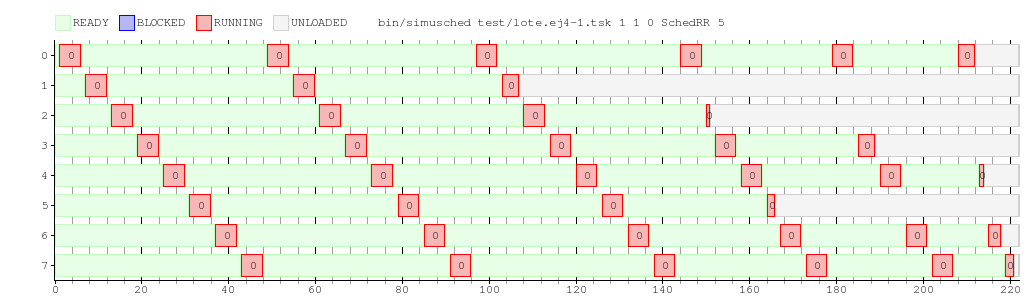
\includegraphics[scale=0.4]{imagenes/ej4-1.png}
\end{center}
\caption{Experimento 1. Lote 8 tareas. Quantum 5.}
\end{figure}

\subsubsection{Conclusión}

\textcolor{red}{\textbf{DEBATIR ESTE PÁRRAFO}}

Como era de esperarse, empieza a ejecutarse el primer proceso \textit{listo}
hasta cumplir su cuota de tiempo, luego pasa a ejecutar al siguiente, y así
hasta retomar la primer tarea (pues se turnan de manera circular). A medida
que los procesos terminan la totalidad de su ejecución, la cola se va
haciendo más corta, acortando el tiempo de espera entre el desalojo de un
proceso y su retorno. Ésto se repite hasta que todos los procesos terminan
su ejecución.

\subsection{Experimento 2: Impacto del quantum}
Con este experimento se logró analizar el impacto del tamaño del quantum en
el tiempo necesario para terminar de ejecutar cada tarea. Asignar un quantum
muy bajo haría que dicho tiempo aumente, dado que habrá más ciclos de
\textit{clock} dedicados a realizar los cambios de contextos, aumentando el
tiempo total que le toma a cada tarea terminar su ejecución,
\textcolor{red}{\textbf{WTF}} pero si este es demasiado alto podría generar
que el tiempo de respuesta percibido sea muy alto, pero como no nos interesa
medir esta métrica, no lo tendremos en cuenta.

Analizaremos primero comparativamente en un procesador de un núcleo, con el
mismo lote de tareas, variando el quantum.

Procesador de 1 núcleo, con un quantum de valor 2.

Procesador de 1 núcleo, con un quantum de valor 7.

Procesador de 1 núcleo, con un quantum de valor 15.

Ahora analizamos comparativamente en un procesador de 4 núcleos, manteniendo
el mismo lote de tareas, y tomando los mismo valores de quantum (en 3
simulaciones distintas).

Procesador de 4 núcleos, con un quantum de valor 2.

Procesador de 4 núcleos, con un quantum de valor 7.

Procesador de 4 núcleos, con un quantum de valor 15.

\subsubsection{Conclusión}

\subsection{Ejercicio 5: Lottery Scheduling}
\subsubsection{Explicación del algoritmo}
El modelo de scheduling \textit{Lottery} consiste en tener un sistema
pseudoaleatorio que decida cual va a ser el siguiente proceso a ser
ejecutado. Esto lo hace \textit{repartiendo tickets} a cada proceso, y
generando un ticket ganador al azar. Así, cada
proceso va a tener asociado una cantidad de tickets, obteniendo
cierta probabilidad de ganar la lotería. De esta forma, el proceso con más
tickets tiene más probabilidades de ganar. Éste es el mecanismo que nos
permite establecer relaciones de prioridades entre procesos.
Y como dado un número entre $1$ y $n$, la posibilidad de que dicho número
\textbf{no} salga nunca es $0$, eventualmente el número será elegido por el
algoritmo de scheduling. De esta forma, no hay \textit{starvation}, pues
todo proceso será puesto a correr en algún momento.

Para implementarlo utilizamos:
\begin{itemize}
\item Una lista de procesos y sus tickets, \textbf{procesos}
%\footnote{Utilizamos \verb|list<pair<int,int> >| de la STL de C++.}.
\item Un diccionario de procesos bloqueados, \textbf{bloqueados}
%\footnote{Utilizamos \verb|map<int,int>| de la STL de C++. }, que dado un pid guarda con cuantos
%tickets tiene que regresar.
\item Una variable entera \textbf{ciclos}, que especifica cuantos ciclos
consumió el proceso actual (el que ocupa el procesador).
\item Una variable entera \textbf{quantum}.
\item Una variable entera \textbf{tickets}, que indica la cantidad de
tickets totales asignados.
\end{itemize}


\section{Ejercicio 6}

\subsection{Explicación del algoritmo}
Para llevar a cabo el algoritmo se precalculó aleatoriamente en que ciclos
de \textit{clock} la tarea debía bloquearse. Para esto reutilizamos la
función \verb|get_rand| utilizada en el ejercicio 1, con el objetivo de
generar un número psudoaleatorio entre 0 y la cantidad de ciclos de cpu en
la que la tarea debe bloquearse.

\newpage

\section{Apéndice 1: acerca de los tests}


\textcolor{red}{\textbf{REVISAR TODO ESTO!}} \medskip

Los \textbf{casos aleatorios se generan mediante los scripts} (en Ruby) \verb|ejN.random.rb|, donde
N es el número correspondiente al problema. Estos scripts toman siempre \textbf{dos parámetros},
siendo el primero la semilla que utilizamos para generar números pseudoaleatorios, que
\textbf{por defecto toma el valor 0} si no es especificado y \textbf{el segundo parámetro corresponde
al tamaño de la entrada}.

Además de los tests con casos aleatorios, \textbf{tenemos en cuenta los mejores y peores
casos de cada algoritmo}, fijando los valores adecuados de los parámetros para
obtenerlos. \medskip

En cuanto a la metodología para medir el tiempo, utilizamos el archivo \verb|tiempo.h|,
que define macros para contar la \textbf{cantidad de ciclos de clock} producidos entre dos instantes. \medskip

Cada instancia se repite varias veces para reducir el impacto de los \textit{outliers}, quedándonos
con el \textbf{valor mínimo} en cada caso. Estos valores (de entrada y salida) se vuelcan a un archivo
\verb|info.n.dat| dentro de la carpeta \textit{benchmark}, que es utilizado luego para generar los gráficos
mediante \textbf{gnuplot}. \medskip

Para correr los tests estáticos (sin variables aleatorias), se ejecuta \verb|make; make test| y para los
casos aleatorios (utilizados para los gráficos), \verb|make; make plot|.

Todos los archivos \verb|.cc| son compilados utilizando la optimización \verb|-O3|. \medskip

Tener en cuenta que, a pesar de ejecutar los tests reiteradas veces, aún es posible que estén presentes ciertos
valores atípicos (menores o mayores a los esperados), ya sea por optimizaciones que realice el procesador, sobrecarga
del mismo, etc.
\newpage

\section{Apéndice 2: secciones relevantes del código}

\textcolor{red}{\textbf{chequear!}} \medskip

En esta sección, adjuntamos parte del código correspondiente a la resolución de cada problema
que consideramos más \textbf{relevante}. Omitimos los encabezados, bibliotecas incluídas,
funciones \verb|main| y de impresión de resultados. El código se encuentra comentado en los
archivos \verb|.cc|.

\subsection{Código del Problema 1}


\begin{lstlisting}
\end{lstlisting}

\vspace*{0.5cm}


\newpage


\subsection{Código del Problema 2}


\begin{lstlisting}
\end{lstlisting}

\vspace*{0.5cm}


\newpage


\subsection{Código del Problema 3}


\begin{lstlisting}
\end{lstlisting}

\vspace*{0.5cm}


\end{document}
